\section{Proposed TNU Tolerant Latch} \label{sec:TNU}

In this section we discuss the implementation of the non-robust triple node upset (TNU) tolerant latch named TNU-latch. We have investigated development of a robust TNU latch but it was exceptionally tedious to verify it correctness. For example, a latch with two more nodes compared to the HRDNUT resulted into nine total nodes and requires the verification of 84 unique cases. Instead, we focused on the development of a simple and efficient non-robust design that has 82 transistors. This design has been verified for all possible TNU cases and is shown to be fully tolerant. 

A schematic of the TNU-latch is given in \ref{fig:TNU}. The latch consists of a base block latch as in the HRDNUT but with 5 storage blocks. Each storage block has a C-element with 4 inputs with each input connected to the other nodes. In addition four of the C-elements have two transistors connected to \textit{CLK} and \textit{CLKB} to ensure that the output node is set to high impedance during the transparent mode. Similar to the HRDNUT, this reduces the power consumption and the delay for a relatively small increase in area. To vote on the output, the nodes in the block latch are connected to two 3-input C-elements which are denoted as \textit{C6} AND \textit{C7} in \ref{fig:TNU}. These C-elements drive a 2-input C-element labeled as \textit{C8}. A schematic of the TNU-latch is given in \ref{fig:TNU}.

\begin{figure}[!tbp]
	\centering
	\includegraphics[width=\linewidth]{Figures/TNULatch}
	%where an .eps filename suffix will be assumed under latex, 
	%and a .pdf suffix will be assumed for pdflatex; or what has been declared
	%via \DeclareGraphicsExtensions.
	\caption{Schematic of the TNU-Latch.}
	\label{fig:TNU}
\end{figure}

The basis behind the latch design is that the C-elements in the block latch cannot be driven to an incorrect value due to a TNU. To ensure this, each C-element has four inputs. If the latch was designed as in the block based latch for the HRDNUT, the output C-element would had five inputs. However, among experimentation with this design it was found that an error on the output element would lead to an unrecoverable error. To solve this issue, the output C-element was split into two 3-input elements which drive a 2-input element. This removed the error since a TNU can, in the worst case, only flip C-element \textit{C6} or \textit{C7} leaving one C-element unaffected thus holding the data. This also allows for the latch to tolerate a TNU with an error on the output since only two errors will affect the internal nodes. None of the C-elements can be flipped due to an internal DNU, thus allowing for the output to recover.

First, we will evaluate the TNU-latch during the transparent mode. In this mode, the data is loaded to nodes \textit{n1}, \textit{n2}, \textit{n3} and \textit{n4} (see Fig. \ref{fig:TNU}). This is done when the clock is at a high value which sets the output node to high impedance and turns on the loading pass gates. Once the four nodes are loaded, all the inputs on C-element \textit{C5} are set such that \textit{n5} is set to the loaded value. Since nodes \textit{n1-n5} are all loaded, C-elements \textit{C6} and \textit{C7} are set thus driving \textit{C8}.

We will now evaluate the latch for tolerance against soft errors. In the case of a SEU, the latch is tolerant since an SEU cannot change the state of a C-element. Additionally, the latch is DNU tolerant for similar reasons. When a TNU occurs, there are 56 total strike cases. Due to the simple design of the latch, we condense all cases into 6 distinct cases which are given in the following list. To verify the cases, waveforms were generated using equation \ref{qeq} and the same simulation parameters as in Section \ref{Proposed} to model the pulse shape for each individual case. The waveforms are given in Figs. \ref{fig:case1}-\ref{fig:case6}.

\begin{enumerate}
	\item This case considers any three strikes on the set of nodes [\textit{n1, n2, n3, n4, n5}]. To demonstrate this case, we consider strikes on nodes \textit{n1}, \textit{n2} and \textit{n3}. While we only discuss this single case, this explanation applies to any combination of nodes that fall in this case. The errors will all propagate to C-element \textit{C5} but will not cause a change on node \textit{n5} since \textit{n4} is not affected. Additionally, the errors will propagate to the inputs of \textit{C1}, \textit{C2}, \textit{C3} and \textit{C4}. However, since at least \textit{n5} will be unaffected, the C-elements will hold their state. Next, we look at C-elements \textit{C6} and \textit{C7} and note that since \textit{n5} does not change values, the C-elements hold the correct value on nodes \textit{n6} and \textit{n7}. Since these nodes have the correct value, node \textit{out} does not change.
	
	\item This case considers a strike on node \textit{out} and any combination of two strikes on nodes within the set [\textit{n1, n2, n3, n4, n5}]. We present the case where nodes \textit{n1}, \textit{n2} and \textit{out} are struck by a TNU. The other instances of TNU for this case will evaluate similarly. The errors on the block latch can be treated as a DNU. Since no additional nodes in the block latch are flipped by the error, the C-elements \textit{C6} and \textit{C7} can only be affected by at most two errors. This implies that neither element will possibly flip due to an error. Since nodes \textit{n6} and \textit{n7} are error-free, \textit{C8} will drive \textit{out} back to the correct state.
	
	\item This case consists of all TNU strikes where the strike affects a single node within the set [\textit{n1, n2, n3, n4, n5}] and strikes on nodes \textit{n6} and \textit{n7}. For simplicity, we only consider the case for errors on \textit{n1}, \textit{n6} and \textit{n7}. All other strike combinations that fall under this case will evaluate similarly. The error on \textit{n1} will propagate to internal elements \textit{n2, n3, n4} and \textit{n5}. However, since only a single error is at the inputs of the C-elements they hold their correct value. Additionally, \textit{C1} is driven back to the error-free value. This allows for nodes \textit{n6} and \textit{n7} to also be recovered. 
	
	\item This case applies to any TNU combination that has two errors from the set [\textit{n1, n2, n3, n4, n5}] and a single error from \textit{n6} or \textit{n7}. As in the previous cases, any TNU falling within this strike combination will evaluate similarly. We present this case by analyzing a TNU striking nodes \textit{n1, n2} and \textit{n6}. The errors on \textit{n1} and \textit{n2} propagate to C-elements \textit{C1, C2, C3, C4} and \textit{C5}. Since each C-element is driven by 4 nodes, no additional nodes flip value. This leads to two of the nodes on \textit{C6} having two erroneous inputs. This ensures that the error on \textit{n6} is not recovered. However, \textit{n7} remains error-free thus allowing the output to be fully recovered. 
	
	\item This case applies to any TNU instance which has one error in the set of [\textit{n1, n2, n3, n4, n5}], a single error on \textit{n6} or \textit{n7}, and an error on \textit{out}. To present the analysis consider errors on nodes \textit{n1}, \textit{n6} and \textit{out}. In this case the error on \textit{n1} will be fully recovered as in case 3. Since the error is recovered, all input nodes to \textit{C6} are error-free allowing for full recovery of the node. \textit{n6} and \textit{n7} are also error-free setting the output of \textit{C8} to the correct value. 
	
	\item Lastly, assume errors on \textit{n6, n7} and \textit{out}. The TNU-latch will fully recover since all of the inputs of \textit{C6} and \textit{C7} are error-free driving nodes \textit{n6} and \textit{n7} to the correct value. The nodes then drive the output of \textit{C8} to the previous error-free value.
	
\end{enumerate}

\begin{figure}[!htbp]
	\centering
	\parbox{4cm}{
		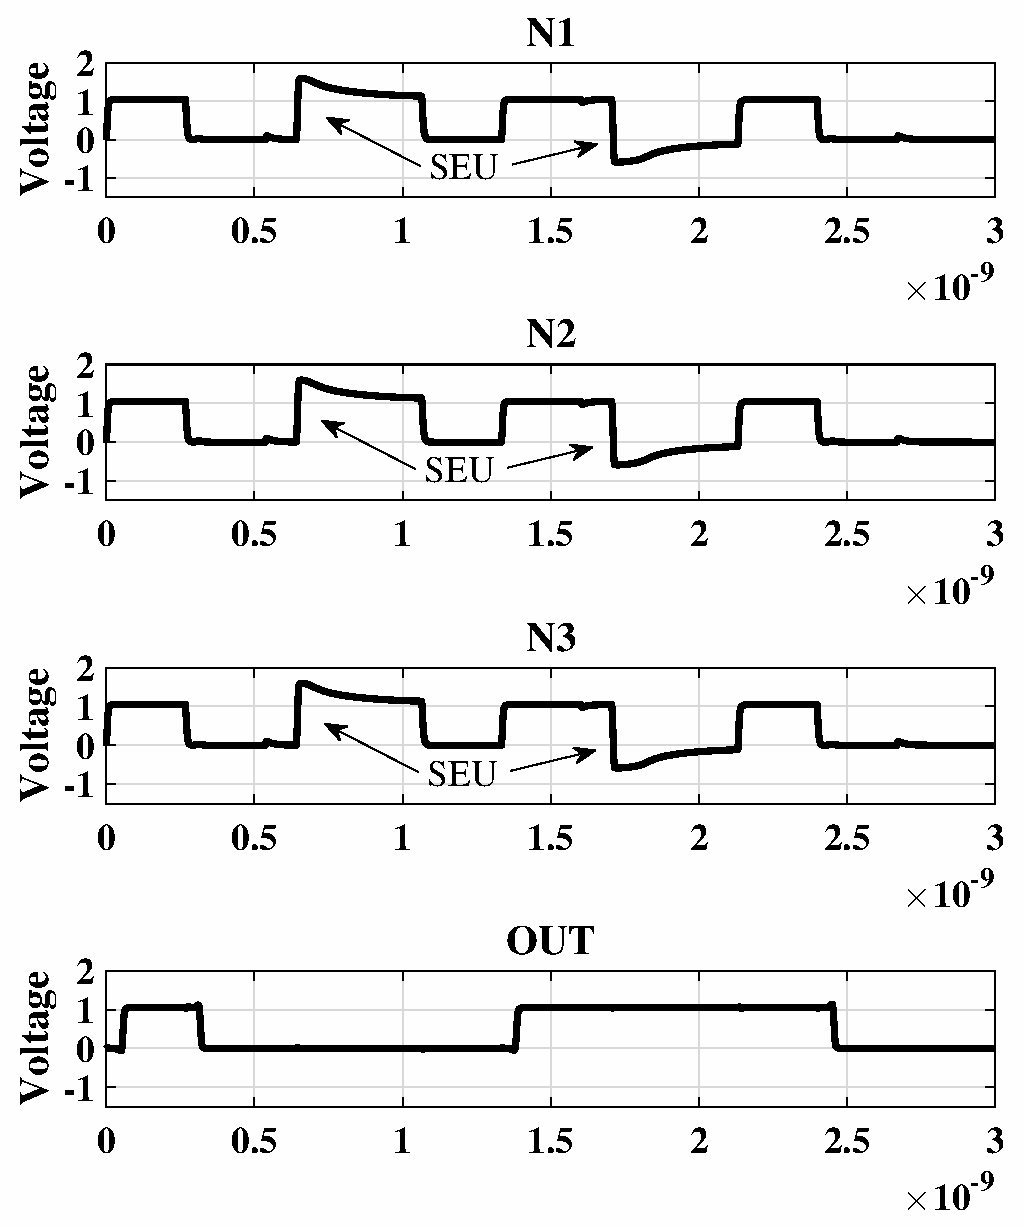
\includegraphics[width=1.15\linewidth]{Figures/TNUPlots/case1.eps}
		\caption{Waveforms for case 1.}
		\label{fig:case1}}
	\qquad
	\begin{minipage}{4cm}
		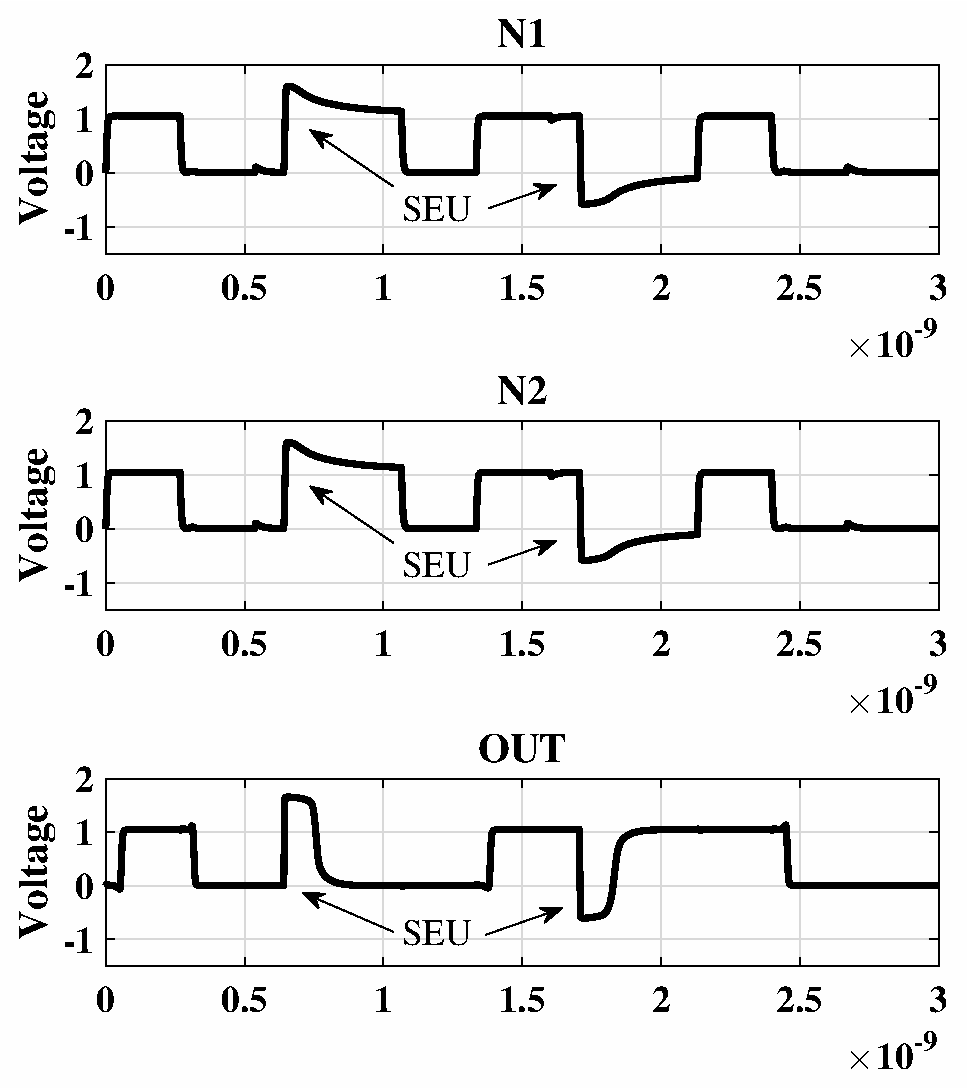
\includegraphics[width=\linewidth]{Figures/TNUPlots/case2.eps}
		\caption{Waveforms for case 2.}
		\label{fig:case2}
	\end{minipage}
\end{figure}

\begin{figure}[!htbp]
	\centering
	\parbox{4cm}{
		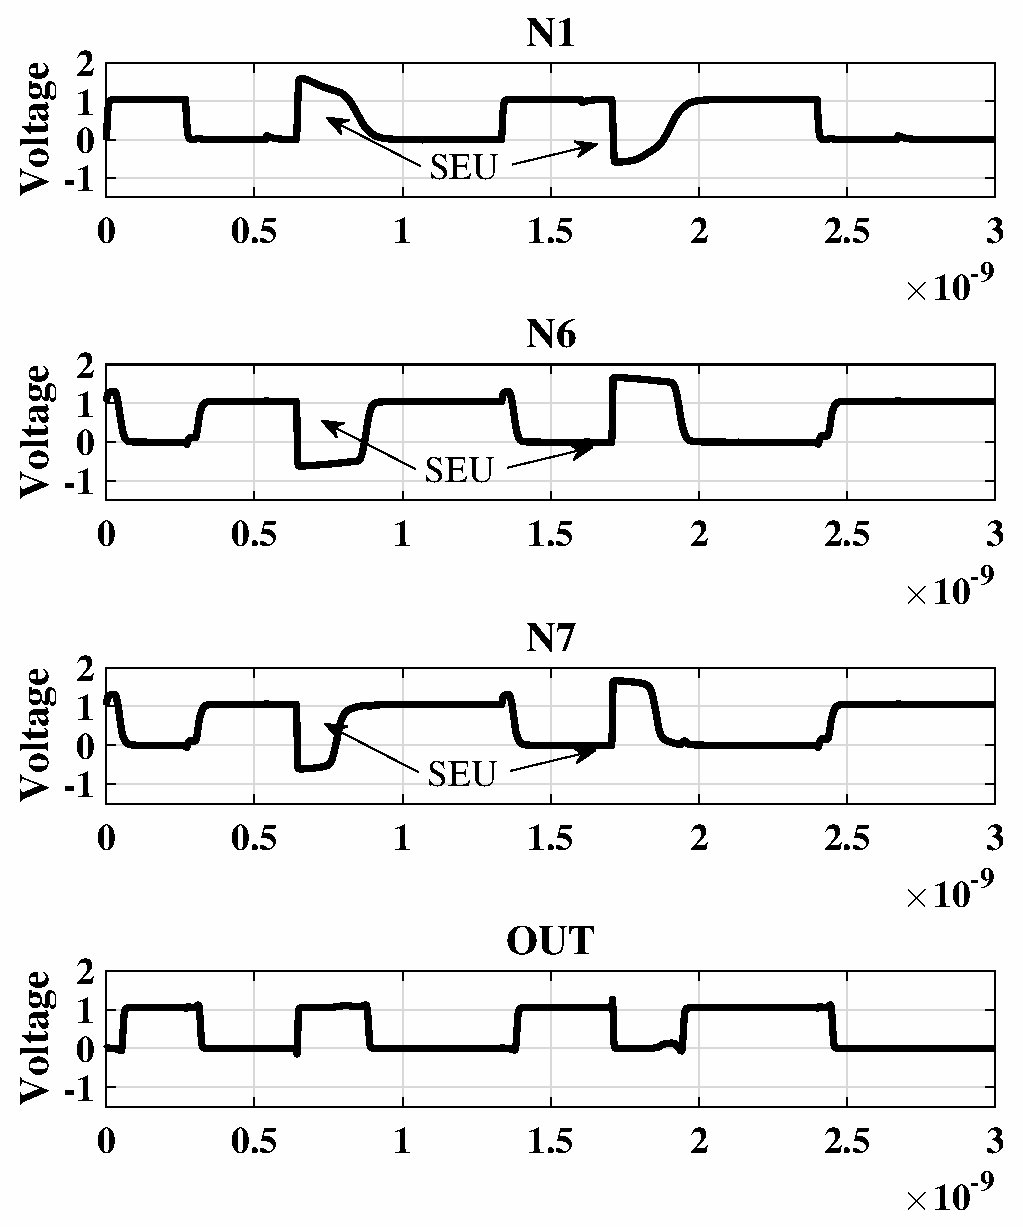
\includegraphics[width=\linewidth]{Figures/TNUPlots/case3.eps}
		\caption{Waveforms for case 3.}
		\label{fig:case3}}
	\qquad
	\begin{minipage}{4cm}
		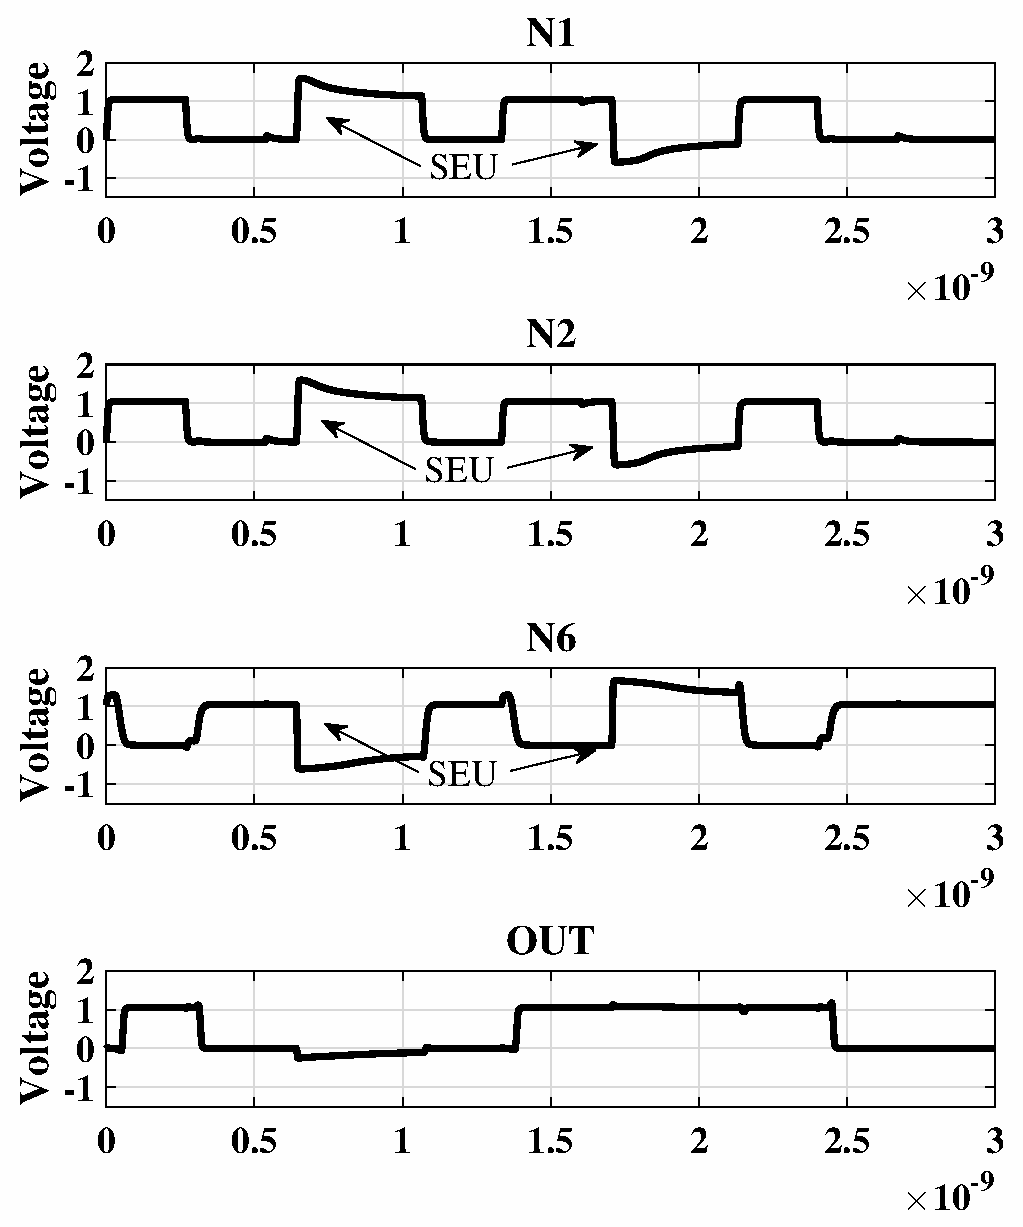
\includegraphics[width=\linewidth]{Figures/TNUPlots/case4.eps}
		\caption{Waveforms for case 4.}
		\label{fig:case4}
	\end{minipage}
\end{figure}

\begin{figure}[!htbp]
	\centering
	\parbox{4cm}{
		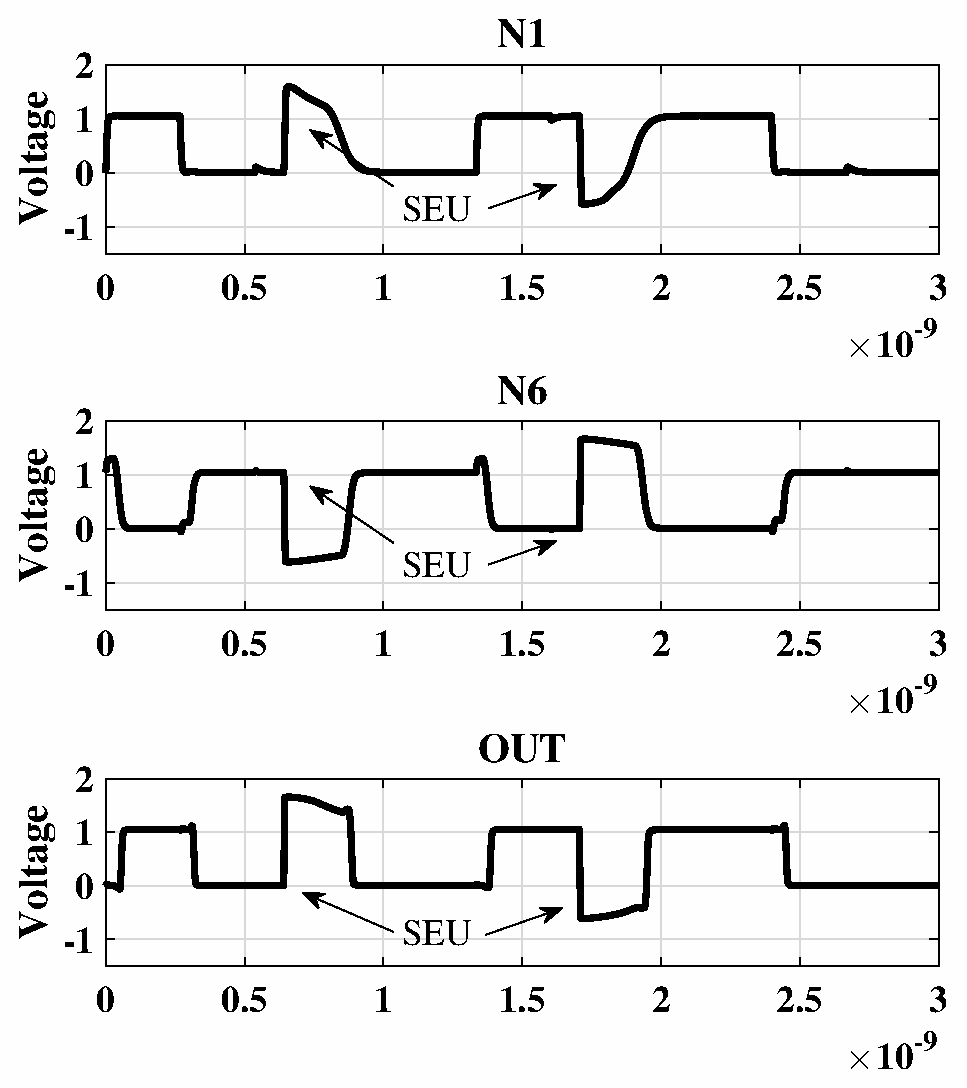
\includegraphics[width=\linewidth]{Figures/TNUPlots/case5.eps}
		\caption{Waveforms for case 5.}
		\label{fig:case5}}
	\qquad
	\begin{minipage}{4cm}
		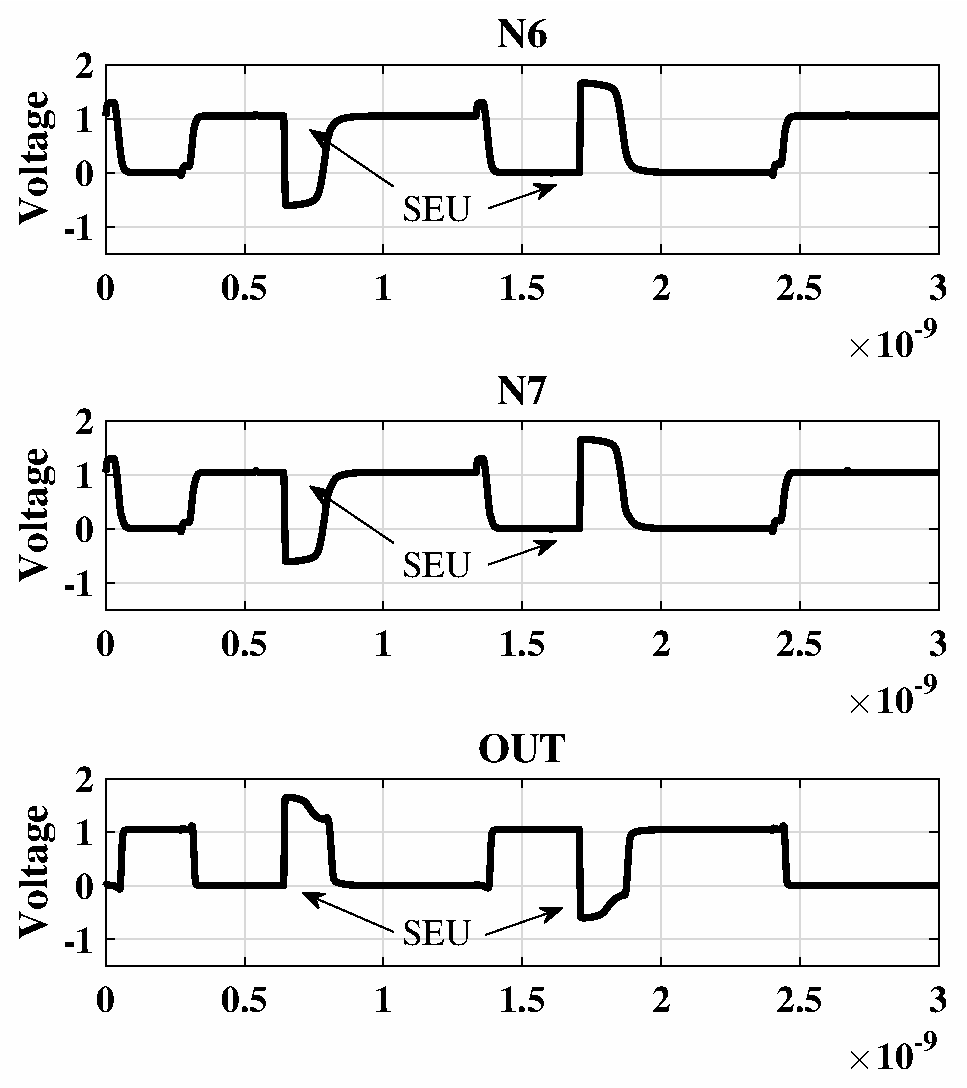
\includegraphics[width=\linewidth]{Figures/TNUPlots/case6.eps}
		\caption{Waveforms for case 6.}
		\label{fig:case6}
	\end{minipage}
\end{figure}